\chapter{HTTP protocol}
HTTP protocol was presented for the first time in the RFC 1945\cite{RFC1945} (Request for Comment).\\
The Hypertext Transfer Protocol (HTTP) is an application-level protocol with the lightness and speed necessary for distributed, collaborative, hypermedia information systems. It is a generic, stateless, object-oriented protocol which can be used for many tasks, such as name servers and distributed object management systems, through extension of its request methods (commands).\\
It's not the first Hypertext protocol in history because there was Hypertalk, made by Apple before. \\
A feature of HTTP is the typing of data representation, allowing systems to be built independently f the data being transferred. HTTP has been in use by the World-Wide Web global information initiative since 1990.

\section{Terminology}
\begin{itemize}
\item{\textbf{connection}\\
a transport layer virtual circuit established between two application programs for the purpose of communication.}
\item{\textbf{message}\\
the basic unit of HTTP communication, consisting of a structured sequence of octets matching the syntax defined in Section 4 and transmitted via the connection.}
\item{\textbf{request}\\
an HTTP request message.
}
\item{\textbf{response}\\
an HTTP response message.}
\item{\textbf{resource}\\
a network data object or service which can be identified by a URI.}
\item{\textbf{entity}\\
a particular representation or rendition of a data resource, or reply from a service resource, that may be enclosed within a request or response message. An entity consists of metainformation in the form of entity headers and content in the form of an entity body.}
\item{\textbf{client}\\
an application program that establishes connections for the purpose of sending requests.}
\item{\textbf{user agent}\\
the client which initiates a request. These are often browsers, editors, spiders (web-traversing robots), or other end user tools.}
\item{\textbf{server}\\
an application program that accepts connections in order to service requests by sending back responses.}
\item{\textbf{origin server}\\
the server on which a given resource resides or is to be created.}
\item{\textbf{proxy}\\
an intermediary program which acts as both a server and a client for the purpose of making requests on behalf of other clients. Requests are serviced internally or by passing them, with possible translation, on to other servers. A proxy must interpret and, if necessary, rewrite a request message before forwarding it.\\
Proxies are often used as client-side portals
through network firewalls and as helper applications for handling requests via protocols not implemented by the user agent.}
\item{\textbf{gateway}\\
a server which acts as an intermediary for some other server. Unlike a proxy, a gateway receives requests as if it were the origin server for the requested resource; the requesting client may not be aware that it is communicating with a gateway.\\
Gateways are often used as server-side portals through network firewalls and as protocol translators for access to resources stored on non-HTTP systems.}
\item{\textbf{tunnel}\\
a tunnel is an intermediary program which is acting as a blind relay between two connections. Once active, a tunnel is not considered a party to the HTTP communication, though the tunnel may have been initiated by an HTTP request. The tunnel ceases to exist when both ends of the relayed connections are closed.\\
Tunnels are used when a portal is necessary and the intermediary cannot, or should not, interpret the relayed communication.}
\item{\textbf{cache}\\
a program's local store of response messages and the subsystem that controls its message storage, retrieval, and deletion. A cache stores cachable responses in order to reduce the response time and network bandwidth consumption on future, equivalent requests. Any client or server may include a cache, though a cache cannot be used by a server while it is acting as a tunnel.}
\end{itemize}
Any given program may be capable of being both a client and a server; our use of these terms refers only to the role being performed by the program for a particular connection, rather than to the program's capabilities in general. Likewise, any server may act as an origin server, proxy, gateway, or tunnel, switching behavior based on the nature of each request.

\section{Basic rules}
The following rules are used throughout are used to describe the grammar used in the RFC 1945.
\begin{table}[h]
\centering
\footnotesize
\begin{tabular}{rl}
\textbf{OCTET =}& <any 8-bit sequence of data>\\
\textbf{CHAR =}& <any US-ASCII character (octets 0 - 127)>\\
\textbf{UPALPHA =}& <any US-ASCII uppercase letter "A".."Z">\\
\textbf{LOALPHA =}& <any US-ASCII lowercase letter "a".."z">\\
\textbf{ALPHA =}& UPALPHA | LOALPHA\\
\textbf{DIGIT =}& <any US-ASCII digit "0".."9">\\
\textbf{CTL =}& <any US-ASCII control character (octets 0 - 31) and DEL (127)>\\
\textbf{CR =}& <US-ASCII CR, carriage return (13)>\\
\textbf{LF =}& <US-ASCII LF, linefeed (10)>\\
\textbf{SP =}& <US-ASCII SP, space (32)>\\
\textbf{HT =}& <US-ASCII HT, horizontal-tab (9)>\\
\textbf{<"> =}& <US-ASCII double-quote mark (34)>\\
\end{tabular}
\end{table}

\section{Messages}
\subsection{Different versions of HTTP protocol}
\begin{itemize}
\item{\textbf{HTTP/0.9 Messages}\\
Simple-Request and Simple-Response do not allow the use of any header information and are limited to a single request method (GET).\\ Use of the Simple-Request format is discouraged because it prevents the server from identifying the media type of the returned entity.
\begin{center}
\begin{tabular}{c}
\begin{lstlisting}[linewidth=240pt, basicstyle=\footnotesize\sffamily,]
HTTP-message = Simple-Request | Simple-Response
\end{lstlisting}
\end{tabular}
\end{center}
\begin{center}
\begin{tabular}{c}
\begin{lstlisting}[linewidth=230pt, basicstyle=\footnotesize\sffamily,]
Simple-Request  = "GET" SP Request-URI CRLF


Simple-Response = [ Entity-Body ]
\end{lstlisting}
\end{tabular}
\end{center}
}
\item{\textbf{HTTP/1.0 Messages}\\
Full-Request and Full-Response use the generic message format of RFC 822 for transferring entities. Both messages may include optional header fields (also known as "headers") and an entity body. The entity body is separated from the headers by a null line (i.e., a line with nothing preceding the CRLF).
\begin{center}
\begin{tabular}{c}
\begin{lstlisting}[linewidth=230pt, basicstyle=\footnotesize\sffamily,]
HTTP-message = Full-Request | Full-Response
\end{lstlisting}
\end{tabular}
\end{center}
\begin{center}
\begin{tabular}{c}
\begin{lstlisting}[linewidth=340pt, basicstyle=\footnotesize\sffamily,]
Full-Request = Request-Line
               *(General-Header | Request-Header | Entity-Header)
               CRLF
               [Entity-Body]


Full-Response = Status-Line
                *(General-Header | Request-Header | Entity-Header)
                CRLF
                [Entity-Body]
\end{lstlisting}
\end{tabular}
\end{center}
}
\end{itemize}

\subsection{Headers}
The order in which header fields are received is not significant. However, it is "good practice" to send General-Header fields first, followed by Request-Header or Response-Header fields prior to the Entity-Header fields.\\
Multiple HTTP-header fields with the same field-name may be present in a message if and only if the entire field-value for that header field is defined as a comma-separated list.
\begin{center}
\begin{tabular}{c}
\begin{lstlisting}[linewidth=260pt, basicstyle=\footnotesize\sffamily,]
HTTP-header = field-name ":" [ field-value ] CRLF
\end{lstlisting}
\end{tabular}
\end{center}

\subsection{Request-Line}
\begin{center}
\begin{tabular}{c}
\begin{lstlisting}[linewidth=320pt, basicstyle=\footnotesize\sffamily,]
Request-Line = Method SP Request-URI SP HTTP-Version CRLF

Method         = "GET" | "HEAD" | "POST" | extension-method

extension-method = token
\end{lstlisting}
\end{tabular}
\end{center}
The list of methods acceptable by a specific resource can change dynamically; the client is notified through the return code of the response if a method is not allowed on a resource.\\
Servers should return the status code 501 (not implemented) if the method is unrecognized or not implemented.

\subsection{Request-URI}
The Request-URI is a Uniform Resource Identifier and identifies the resource upon which to apply the request.
\begin{center}
\begin{tabular}{c}
\begin{lstlisting}[linewidth=190pt, basicstyle=\footnotesize\sffamily,]
Request-URI = absoluteURI | abs_path
\end{lstlisting}
\end{tabular}
\end{center}
The absoluteURI form is only allowed when the request is being made to a proxy. The proxy is requested to forward the request and return the response. If the request is GET or HEAD and a prior response is cached, the proxy may use the cached message if it passes any restrictions in the Expires header field.\\
Note that the proxy may forward the request on to another proxy or directly to the server specified by the absoluteURI. In order to avoid request loops, a proxy must be able to recognize all of its server names, including any aliases, local variations, and the numeric IP address.\\\\
The most common form of Request-URI is that used to identify a resource on an origin server or gateway. In this case, only the absolute path of the URI is transmitted.

\subsection{Request Header}
The request header fields allow the client to pass additional information about the request, and about the client itself, to the server.\\
These fields act as request modifiers, with semantics equivalent to the parameters on a programming language method (procedure) invocation.
\begin{center}
\begin{tabular}{c}
\begin{lstlisting}[linewidth=410pt, basicstyle=\footnotesize\sffamily,]
Request-Header = Authorization | From | If-Modified-Since | Referer | User-Agent
\end{lstlisting}
\end{tabular}
\end{center}

\subsection{Status line}
\begin{center}
\begin{tabular}{c}
\begin{lstlisting}[linewidth=330pt, basicstyle=\footnotesize\sffamily,]
Status-Line = HTTP-Version SP Status-Code SP Reason-Phrase CRLF
\end{lstlisting}
\end{tabular}
\end{center}
\begin{table}[h]
\centering
\footnotesize
\begin{tabular}{|r|l|}
\multicolumn{2}{c}{\textbf{General Status code}}\\
\hline
\textbf{1xx: Informational} & {Not used, but reserved for future use}\\
\hline
\textbf{2xx: Success}&{The action was successfully received,}\\
\hline
& {understood, and accepted.}\\
\hline
\textbf{3xx: Redirection} & {Further action must be taken in order to}\\
&{complete the request}\\
\hline
\textbf{4xx: Client Error}&{The request contains bad syntax or cannot}\\
&{be fulfilled}\\
\hline
\textbf{5xx: Server Error}&{The server failed to fulfill an apparently}\\
&{valid request}\\
\hline
\end{tabular}
\end{table}
\begin{table}[h]
\centering
\footnotesize
\begin{tabular}{|r|l|}
\multicolumn{2}{c}{\textbf{Known service code}}\\
\hline
\textbf{200}&{OK}\\
\hline
\textbf{201}&{Created}\\
\hline
\textbf{202}&{Accepted}\\
\hline
\textbf{204}&{No Content}\\
\hline
\textbf{301}&{Moved Permanently}\\
\hline
\textbf{302}&{Moved Temporarily}\\
\hline
\textbf{304}&{Not Modified}\\
\hline
\textbf{400}&{Bad Request}\\
\hline
\textbf{401}&{Unauthorized}\\
\hline
\textbf{403}&{Forbidden}\\
\hline
\textbf{404}&{Not Found}\\
\hline
\textbf{500}&{Internal Server Error}\\
\hline
\textbf{501}&{Not Implemented}\\
\hline
\textbf{502}&{Bad Gateway}\\
\hline
\textbf{503}&{Service Unavailable}\\
\hline
\end{tabular}
\end{table}

\section{HTTP 1.0}
The protocol has no mandatory headers to be added in the request field. This protocol is compliant with HTTP 0.9.
To keep the connection alive, "Connection" header with "keep-alive" as header field must be added to request message. The server, receiving the request, replies with a message with the same header value for "Connection".\\
This is used to prevent the closure of the connection, so if the client needs to send another request, he can use the same connection.
This is usually used to send many files and not only one.\\
The connection is kept alive until either the client or the server decides that the connection is over and one of them drops the connection. If the client doesn't send new requests to the server, the second one usually drops the connection after a couple of minutes.\\
The client could read the response of request, with activated keep alive option, reading only header and looking to "Content-length" header field value to understand the length of the message body. This header is added only if a request with keep-alive option is done.\\
This must be done because we can't look only to empty system stream, because it could be that was send only the response of the first request or a part of the response.\\
Otherwise, when the option keep alive is not used, the client must fix a max number of characters to read from the specific response to his request, because he doesn't know how many character compose the message body. If you make many requests to server without keep-alive option, the server will reply requests, after the first, with only headers but empty body.\\

\subsection{Other headers of HTTP/1.0 and HTTP/1.1}
\begin{itemize}
\item{\textbf{Allow}\\
lists the set of HTTP methods supported by the resource identified by the Request-URI}
\item{\textbf{Accept}\\
lists what the client can accept from server. It's important in object oriented typing concept because client application knows what types of data are allowed for its methods or methods of used library}\\
\item{\textbf{Accept-encoding}\\
specifies what type of file encoding the client supports (don't confuse it with transfer encoding)}\\
\item{\textbf{Accept-language}\\
specifies what language is set by Operating System or it's specified as a preference by client on browser}\\
\item{\textbf{Content-Type}\\
indicates the media type of the Entity-Body sent to the recipient. It is often used by server to sppecify which one of the media types, indicated by the client in the Accept request, it will use in the response.}
\item{\textbf{Date}\\
specifies the date and time at which the message was originated}
\item{\textbf{From}\\
if given, it should contain an Internet e-mail address for the human user who controls the requesting user agent (it was used in the past)}
\item{\textbf{Location}\\
defines the exact location of the resource that was identified by the Request-URI (useful for 3xx responses)}
\item{\textbf{Pragma}\\
It's sent by server to inform that there in no caching systems}\\
\item{\textbf{Referer}\\
allows the client to specify, for the server's benefit, the address (URI) of the resource from which the Request-URI was obtained (page from which we clicked on the link). This allows a server to generate lists of back-links to resources for interest, logging, optimized caching, etc.
It was added with the born of economy services related to web pages.}
\item{\textbf{Server}\\
information about the software used by the origin server to handle the request (usually Apache on Unix, GWS(Google Web Server), Azure on Windows, ...)}
\item{\textbf{User-agent}\\
Version of client browser and Operating System. It's used to:
\begin{itemize}
\item{adapt responses to application library}
\item{manage mobile vs desktop web pages}
\end{itemize}
It's crucial for web applications. If we are the clients and we receive the response from server, we want that the content must change according to the version of browser. \\
Infact, there are two different web pages(two different view of the same web page) according to connection by pc and phone, because of different user-agent of these devices. If a mobile phone sends a request to a non-mobile web page, the user agent changes to user agent related to Desktop version.}\\
\end{itemize}

\subsection{Caching}
It's based on locality principle and was observed on programs execution.
\begin{itemize}
\item{\textbf{Time Locality}\\
When a program accesses to an address, there will be an access to it again in the near future with high probability.\\
If I put this address in a faster memory (cache), the next access to the same location would be faster.
\begin{figure}[h]
\centering
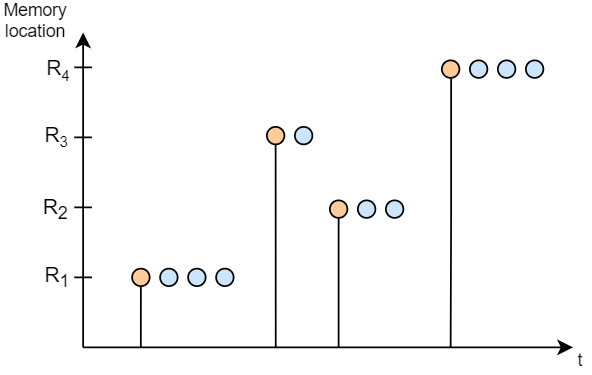
\includegraphics[scale=0.5]{Images/HTTP/time_locality}
\end{figure}
}
\item{\textbf{Space Locality}\\
If a program accesses to an address in the memory, it's very probable that neighboring addresses would be accessed next.}
\end{itemize}
The caching principle is applied also in Computer Networks, storing of the visited web pages on client system and then updating them through the use of particular headers and requests (see Figure \ref{caching}). The purpose of using cache is to reduce traffic over the network and load of the server. The main problem of storing the page in a file, used as a cache, is that the page on the server can me modified and so client's copy can be obsolete.\\
\begin{figure}[h]
\centering
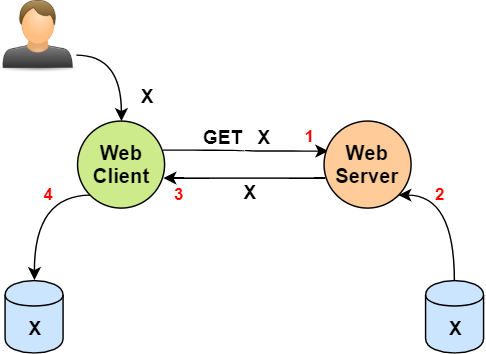
\includegraphics[scale=0.5]{Images/HTTP/caching}
\caption{\footnotesize{First insertion of the resource in the cache.\\}}\label{catching}
\end{figure}
The update of the content of the local cache for the client can happen in three different ways:
\begin{itemize}
\item{\textbf{Expiration date}
\begin{enumerate}
\item{The client asks the resource to the server, that replies with the resource and adding "Expires" header. This is done by the server to specify wan the resource will be considered obsolete.}
\item{The client stores a copy of the resource in its local cache.}
\item{The client, before sending a new request, checks if it has already the resource he's asking to server. If he has already the resource, he compares the Expiration date, specified by server at phase 1, with the real time clock. }
A problem of this method is that the server needs to know in advance when the page changes. So the "Expires" value, sent by server, must be:
\begin{itemize}
\item{exactly known in advance for periodic changes (E.g. daily paper)}
\item{statistically computed (evaluating the probability of refreshing and knowing a lower bound of duration of resource)}
\end{itemize}
The other problem of this method is that we need to have server and client clocks synchronized. Hence, we need to have date correction and compensation between these systems.
\end{enumerate}
\begin{figure}[h]
\centering
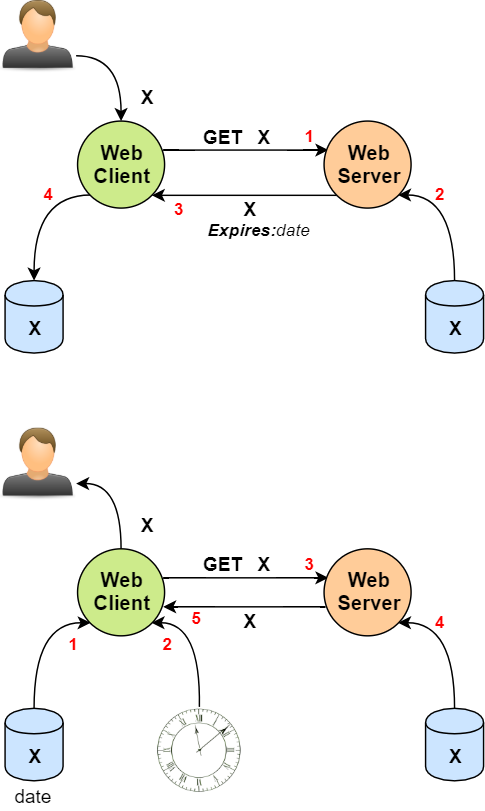
\includegraphics[scale=0.5]{Images/HTTP/expires_cache}
\end{figure}
}
\clearpage
\item{\textbf{Request of only header part}
\begin{enumerate}
\item{The client asks the resource to the server as before but now, he stores resource in the cache, within also its "Last-Modified" header value.}
\item{The client checks if its copy of the resource is obsolete by making a request to the server of only the header of the resource. This type of request is done by using the \textit{"HEAD"} method.}
\item{The client looks to the value of the header "Last-Modified", received by the server. This value is compared with the last-modified header value stored within the resource. \\
If the store date was older than new date, the client makes a new request for the resource to the server. Otherwise, he uses the resource in the cache.}
\end{enumerate}
The problem of this method is that, in the worst case, we send two times the request of the same resource (even if the first one, with "HEAD" method, is less heavy).
\begin{figure}[h]
\centering
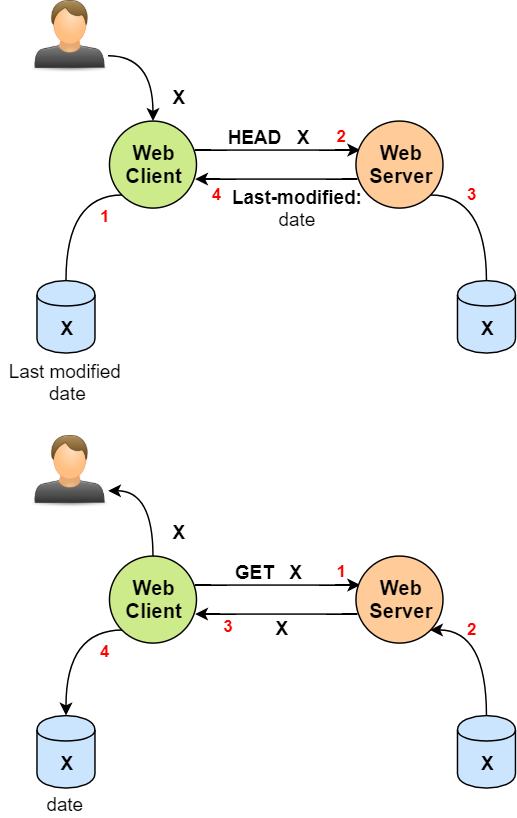
\includegraphics[scale=0.5]{Images/HTTP/last_cache}
\end{figure}
}
\clearpage
\item{\textbf{Request with if-modified-since header}\\
\begin{enumerate}
\item{The client asks the resource to the server as before, storing the resource in the cache within its "Last-Modified" header value.}
\item{When the client needs again the resource, it sends the request to the server, specifying also "If-Modified-Since" header value as store data.
}
\item{If the server, looking to the resource, sees that its Last-Modified value is more recent than date specified in the request by client, it sends back to the recipient the newer resource.\\
Otherwise, it sends to client the message "HTTP/1.0 304 Not Modified".}
\end{enumerate}
The positive aspect of this method is that the client can do only a request and obtain the corrept answer without other requests.
\begin{figure}[h]
\centering
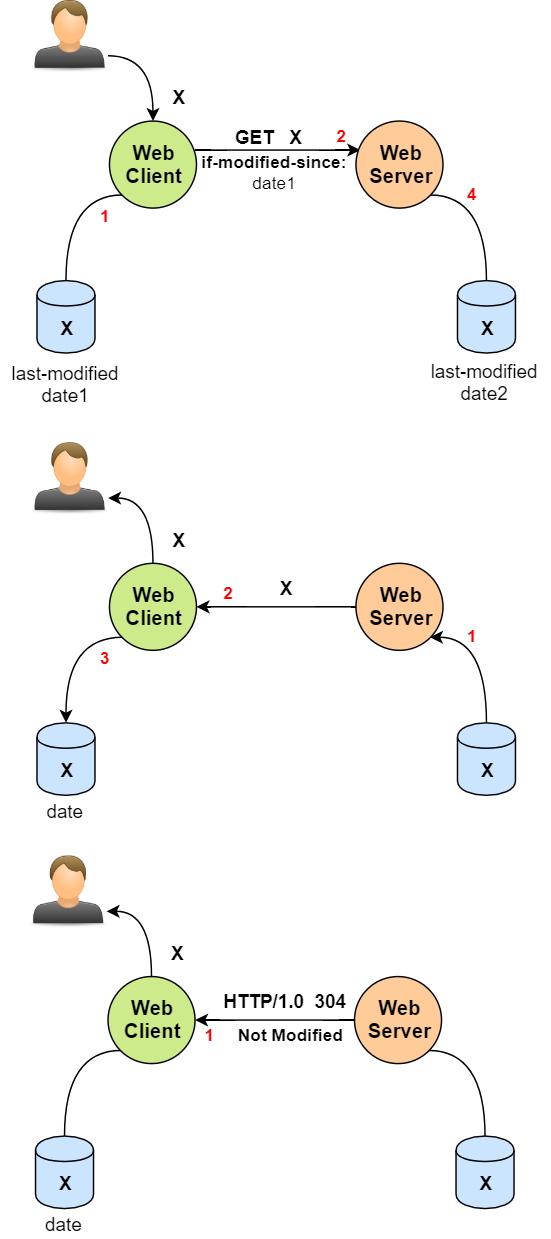
\includegraphics[scale=0.5]{Images/HTTP/if_cache}
\end{figure}
}
\end{itemize}
\clearpage
\subsection{Authorization}
\begin{enumerate}
\item{The client sends the request of the resource to the client}
\item{The server knows that the resource, to be accessible, needs the client authentication, so it sends the response specifying "WWW-Authenticate:" header, as the following:
\begin{center}
\begin{tabular}{c}
\begin{lstlisting}[linewidth=220pt, basicstyle=\footnotesize\sffamily,]
WWW-Authenticate: Auth-Scheme Realm="XXXX"
\end{lstlisting}
\end{tabular}
\end{center}
\begin{table}[h]
\centering
\footnotesize
\begin{tabular}{rl}
\textbf{Auth-Scheme}& {Type of encryption adopted}\\
\textbf{Realm}& {"XXXX" refering to the set of users that can access to the resource}\\
\end{tabular}
\end{table}
}
\item{The client replies with another request of the same resource but specifying also the "Authorization" header value, as the following:
\begin{center}
\begin{tabular}{c}
\begin{lstlisting}[linewidth=220pt, basicstyle=\footnotesize\sffamily,]
WWW-Authenticate: Auth-Scheme Basic-cookie
\end{lstlisting}
\end{tabular}
\end{center}
\begin{table}[h]
\centering
\footnotesize
\begin{tabular}{rl}
\textbf{Auth-Scheme}& {Type of encryption adopted}\\
\textbf{Basic-cookie}& {Base64 encrypted message of the needed for the authentication}\\
{}&{(in general basic-ccokie doesn't contain password inside it, it happens only in this case)}
\end{tabular}
\end{table}
}
\end{enumerate}
\begin{figure}[h]
\centering
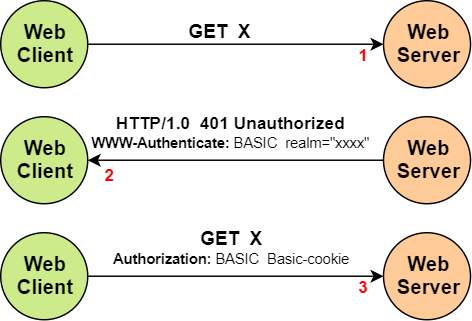
\includegraphics[scale=0.5]{Images/HTTP/auth}
\end{figure}
\clearpage
\subsubsection{base64}
It is very useful for a lot of protocol like HTTP, that doesn't support format different than text of characters. For example with SMTP, all the mail contents must be text, hence images or other binary files are encrypted with base64.\\
Starting from a stream of bytes, we are going to convert numbers, described by each byte, into ANSI character symbols. These selected symbols, from the Table \ref{base64_table} of all the 64 symbols, are generated looking the values of subsequences of 6 bits.\\
If the stream of bytes is not composed by a multiple of 24 bits, base64 pad whole missing bytes with symbol '=' (not defined as one of the 64 symbols of the alphabet) and other single missing bits with 0 values.
\begin{figure}[h]
\centering
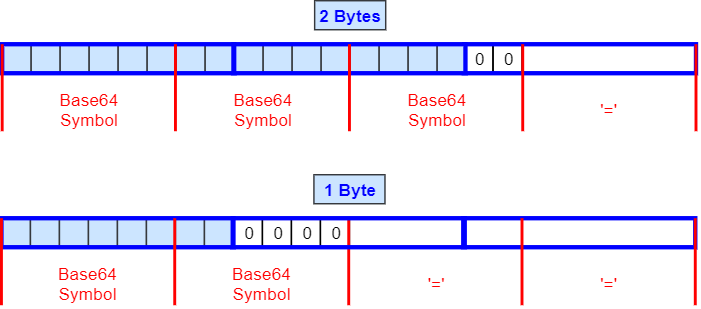
\includegraphics[scale=0.5]{Images/HTTP/pad_base64}
\end{figure}
\begin{figure}[h]
\centering
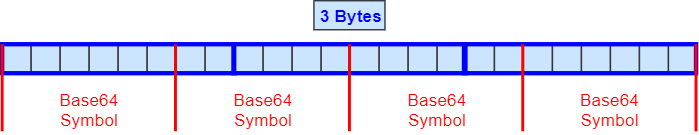
\includegraphics[scale=0.5]{Images/HTTP/base64}
\end{figure}
\vspace{1cm}

\begin{table}[h]
\footnotesize\centering
\begin{tabular}{|rlcrlcrlcrl|}
\hline
 {0 }&{A}&{   }&{16 }&{Q}&{   }&{32 }&{g}&{   }&{48 }&{w}\\
 {1 }&{B}&     &{17 }&{R}&     &{33 }&{h}&     &{49 }&{x}\\
 {2 }&{C}&     &{18 }&{S}&     &{34 }&{i}&     &{50 }&{y}\\
 {3 }&{D}&     &{19 }&{T}&     &{35 }&{j}&     &{51 }&{z}\\
 {4 }&{E}&     &{20 }&{U}&     &{36 }&{k}&     &{52 }&{0}\\
 {5 }&{F}&     &{21 }&{V}&     &{37 }&{l}&     &{53 }&{1}\\
 {6 }&{G}&     &{22 }&{W}&     &{38 }&{m}&     &{54 }&{2}\\
 {7 }&{H}&     &{23 }&{X}&     &{39 }&{n}&     &{55 }&{3}\\
 {8 }&{I}&     &{24 }&{Y}&     &{40 }&{o}&     &{56 }&{4}\\
 {9 }&{J}&     &{25 }&{Z}&     &{41 }&{p}&     &{57 }&{5}\\
{10 }&{K}&     &{26 }&{a}&     &{42 }&{q}&     &{58 }&{6}\\
{11 }&{L}&     &{27 }&{b}&     &{43 }&{r}&     &{59 }&{7}\\
{12 }&{M}&     &{28 }&{c}&     &{44 }&{s}&     &{60 }&{8}\\
{13 }&{N}&     &{29 }&{d}&     &{45 }&{t}&     &{61 }&{9}\\
{14 }&{O}&     &{30 }&{e}&     &{46 }&{u}&     &{62 }&{+}\\
{15 }&{P}&     &{31 }&{f}&     &{47 }&{v}&     &{63 }&{/}\\
\hline
&&&&&{pad =}&&&&&\\
\hline
\end{tabular}
\end{table}

\subsubsection{Auth-schemes}
\begin{itemize}
\item{\textbf{BASIC}\\
\begin{figure}[h]
\centering
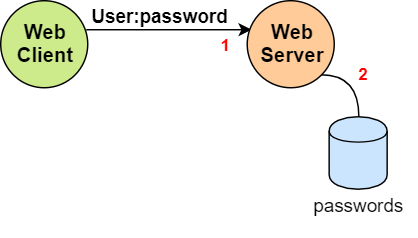
\includegraphics[scale=0.5]{Images/HTTP/basic}
\end{figure}
}
\item{\textbf{Challenge} (symmetric version)\\
\begin{figure}[h]
\centering
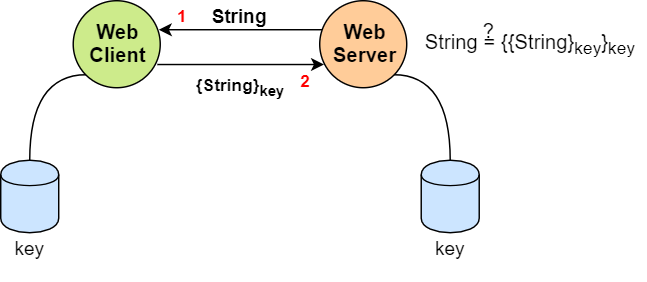
\includegraphics[scale=0.5]{Images/HTTP/challenge_sym}
\end{figure}
}
\item{\textbf{Challenge} (asymmetric version)\\
\begin{figure}[h]
\centering
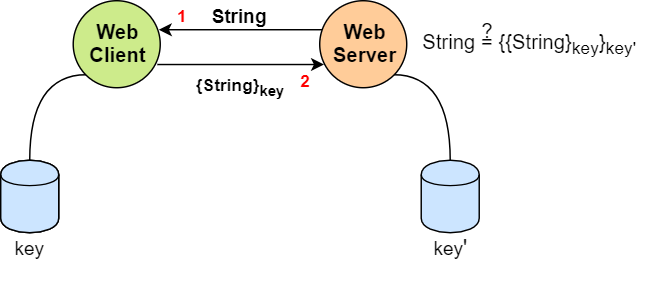
\includegraphics[scale=0.5]{Images/HTTP/challenge_asym}
\end{figure}
}
\end{itemize}
\section{HTTP 1.1}
It has by default the option keep alive actived by default with respect to HTTP 1.0. It has the mandatory header "Host" followed by the hostname of the remote system, to which the request or the response is sent. The headers used in HTTP/1.0 are used also in HTTP/1.1, but in this new protocol there are new headers not used in the previous one. The body is organized in chunks, so we need the connection kept alive to manage future new chunks.\\
This is useful with dynamic pages, in which the server doesn't know the length of the stream in advance and can update the content of the stream during the extablished connection, sending a fixed amount of bytes to client. We can check if the connection is chunked oriented, looking for the header "Transfer-Encoding" with value "chunked".\\
Each connection is composed by many chunks and each of them is composed by chunk length followed by chunk body, except for the last one that has length 0 (see Figure \ref{chunked_body}). The following grammar represents how the body is organized:
\begin{center}
\begin{tabular}{c}
\begin{lstlisting}[linewidth=320pt, basicstyle=\footnotesize\sffamily,]
Chunked-Body   = *chunk
                 last-chunk
                 trailer
                 CRLF

chunk          = chunk-size [ chunk-extension ] CRLF
                 chunk-data CRLF

chunk-size     = 1*HEX
last-chunk     = 1*("0") [ chunk-extension ] CRLF

chunk-extension= *( ";" chunk-ext-name [ "=" chunk-ext-val ] )

chunk-ext-name = token
chunk-ext-val  = token | quoted-string
chunk-data     = chunk-size(OCTET)
trailer        = *(entity-header CRLF)
\end{lstlisting}
\end{tabular}
\end{center}

\begin{figure}[h]
\centering
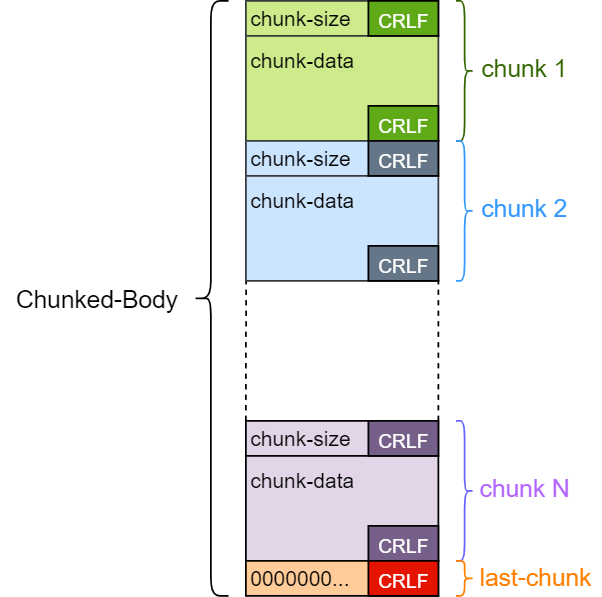
\includegraphics[scale=0.5]{Images/HTTP/Chunked-Body}\caption{\footnotesize{Chunked body.}}\label{chunked_body}
\end{figure}

\subsection{Caching based on HASH}
It's like the caching mechanism used looking to "Last-Modified" header value through the use of HEAD. The organization is as follows:
\begin{enumerate}
\item{The client asks the resource to the server, he stores resource in the cache, within also its "Etag" header value.}
\item{The client checks if its copy of the resource is obsolete by making a request to the server of only the header of the resource. This type of request is done by using the \textit{"HEAD"} method.}
\item{The client looks to the value of the header "Etag", received by the server. This value is compared with the "Etag" header value stored within the resource, because everytime that a file changes, its hash code is computed again.\\
If the store date has different hash code from one received, the client makes a new request for the resource to the server. Otherwise, he uses the resource in the cache.}
\end{enumerate}

\subsection{URI}
In URI, there is the encapsulation of the operation done in the past, to have a resource from a server. The following phases are related to \textbf{ftp} application:
\begin{enumerate}
\item{Open the application ftp}
\item{Open the server File System, through a general login}
\item{Select the resource you want to use and download it}
\end{enumerate}
\begin{center}
\begin{tabular}{c}
\begin{lstlisting}[linewidth=320pt, basicstyle=\footnotesize\sffamily,]
URI            = ( absoluteURI | relativeURI ) [ "#" fragment ]

absoluteURI    = scheme ":" *( uchar | reserved )
relativeURI    = net_path | abs_path | rel_path

net_path       = "//" net_loc [ abs_path ]
abs_path       = "/" rel_path
rel_path       = [ path ] [ ";" params ] [ "?" query ]

path           = fsegment *( "/" segment )
fsegment       = 1*pchar
segment        = *pchar

params         = param *( ";" param )
param          = *( pchar | "/" )

scheme         = 1*( ALPHA | DIGIT | "+" | "-" | "." )
net_loc        = *( pchar | ";" | "?" )
query          = *( uchar | reserved )
fragment       = *( uchar | reserved )

pchar          = uchar | ":" | "@" | "&" | "=" | "+"
uchar          = unreserved | escape
unreserved     = ALPHA | DIGIT | safe | extra | national

escape         = "%" HEX HEX
reserved       = ";" | "/" | "?" | ":" | "@" | "&" | "=" | "+"
extra          = "!" | "*" | "'" | "(" | ")" | ","
safe           = "$" | "-" | "_" | "."
unsafe         = CTL | SP | <"> | "#" | "%" | "<" | ">"
national       = <any OCTET excluding ALPHA, DIGIT,
\end{lstlisting}
\end{tabular}
\end{center}
Hence Uniform Resource Identifiers are simply formatted strings which identify--via name, location, or any other characteristic--a network resource. The following example refers to Relative URI:
\begin{center}
\begin{tabular}{c}
\begin{lstlisting}[linewidth=320pt, basicstyle=\footnotesize\sffamily,]
//net_loc/a/b/c?parameters
\end{lstlisting}
\end{tabular}
\end{center}
\begin{table}[h]
\centering \footnotesize
\begin{tabular}{rl}
\textbf{//net\_loc}&{Server location}\\
\textbf{/a/b/c}&{Resource with the path}\\
\textbf{?parameters}&{Set of parameters}
\end{tabular}
\end{table}

\subsection{HTTP URL}
It's a particulare instance of absolute URI, with scheme "http".
\begin{center}
\begin{tabular}{c}
\begin{lstlisting}[linewidth=320pt, basicstyle=\footnotesize\sffamily,]
http_URL       = "http:" "//" host [ ":" port ] [ abs_path ]

host           = <A legal Internet host domain name
                  or IP address (in dotted-decimal form),
                  as defined by Section 2.1 of RFC 1123>

port           = *DIGIT
\end{lstlisting}
\end{tabular}
\end{center}
There are also other schemes that are not used for web, for example \textbf{ftp} to download resources.

\section{Dynamic pages}
Dynamic pages are created on fly by some web applications in the server. The client makes a request to the server function with some parameters (Figure \ref{cgi}).\\
This approach is based on \textbf{Common Gateway Interface (CGI-bin)}, whose name comes from first network applications that were binary. Then the evolution of web applications brings to two types of program:
\begin{itemize}
\item{\textbf{Script Server programs}\\
based on PHP, ASP.net}
\item{\textbf{Server application (based on Java)}
written through J2EE, TomCat and Websphere}
\end{itemize}
The result of these programs are written at Presentation layer, like HTML source. To use the CGI-bin paradigm, the client needs to create a request for a file to be executed and not transfered. For convention, the server usually has its executable files in \textbf{"/CGI-bin"} path of the server.
The following HTTP URL is the request to the server, made by the client, for the function \textbf{f}:
\begin{center}
\begin{tabular}{c}
\begin{lstlisting}[linewidth=280pt, basicstyle=\footnotesize\sffamily,]
http://www.hello.com/CGI-bin/f?a=10&b=20&c=%22ciao%22
\end{lstlisting}
\end{tabular}
\end{center}
In this example the client is asking to server \textbf{www.hello.com}, using an HTTP URL, the result of the call of function \textbf{f}. The symbol \textbf{?} defines from which point the parameters of the function are specified. In this case there are three parameters: \textbf{a} with value \textbf{10}, \textbf{b} with value \textbf{20} and \textbf{c} with value \textbf{\%22ciao\%22}.\\ There are particular symbols, used in URL:
\begin{table}[h]
\centering \footnotesize
\begin{tabular}{|l|l|}
\hline
\textbf{?}&{Beginning of parameters section}\\
\hline
\multirow{2}{*}{\textbf{\%}}&{\textit{Escape character}}\\
&{followed by the hex number that defines the symbol you want to code}\\
\hline
\multirow{2}{*}{\textbf{\&}}&{\textit{Separator character}}\\
&{character between each couple of specified parameters}\\
\hline
\end{tabular}
\end{table}
\begin{figure}[ht]
\centering
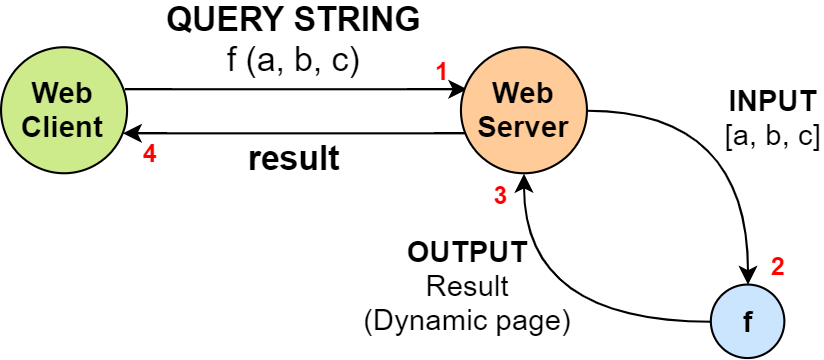
\includegraphics[scale=0.4]{Images/HTTP/cgi}
\caption{\footnotesize{Example of CGI application.}}\label{cgi}
\end{figure}